%!TEX root=./report.tex
\section{EVALUATION}

As a reminder, our task is identifying the correct object model from a large database, given a scan of a model in an uncluttered scene.
The detector should output one answer to this problem, although we also evaluate the process by which it arrives at the final answer.
In our evaluations, we care about both accuracy and speed of the detector.

\subsection{Accuracy Dashboard}

We evaluate the correctness of our results via the following scalar values
\begin{itemize}
  \item Percentage of final results that are correct. This gives a rough idea of how well the detector is performing.
  \item The Average Precision (AP), which is the area under the Precision-Recall curve for the registration accuracy of the final result. The AP is one of the most common scalar metrics of performance in computer vision~\cite{pascal-voc-2010}.
  \item Average rank of correct model (using preliminary voting results). This number speaks to how well the features can get the right answer without any registration steps.
  \item Area under the cumulative result-within-top-K histogram (using preliminary voting results). This gives a complementary picture to the average rank, as it describes the shape of the histogram instead of merely its mean. The maximum value is $1$, and the minimum value is $0.5$.
\end{itemize}

These scalar metrics, in table form, form one part of our Accuracy Dashboard, seen in~\autoref{fig:PSB_dashboard}.
The idea of the Dashboard is that each run of Proctor generates this complete set of results, all available in one place.
Proctor outputs all figures and data for the dashboard, and generates an HTML page or a PDF document tying them together.
In fact, ~\autoref{fig:PSB_dashboard} is an example of such an automatically-generated document.

The results for the Princeton Shape Benchmark can be seen in~\autoref{tab:PSB_results}

In addition, we evaluate more qualitatevly by visualizing the confusion matrix between final results, and through plotting the Precision-Recall curves.
These visualizations are also part of the dashboard, as seen in~\autoref{fig:PSB_dashboard}.

\begin{figure*}[thpb]
\centering
  \subfloat[Table of scalar measures of performance. The best number in each row is emphasized.]{
\label{tab:PSB_results}
\begin{tabular}{ | l || c | c | c | c | }
\hline
Metric & PFH & FPFH & SHOT & Spin \\
\hline
 \% Correct & 86.25 & \bf 87.50 & 73.75 & 49.35 \\
AP & 0.85 & \bf 0.86 & 0.64 & 0.31 \\
Avg. Rank & 2.23 & \bf 2.16 & 2.23 & 3.45 \\
AUCR & 0.85 & \bf 0.85 & 0.85 & 0.65 \\
\hline
\end{tabular}
  } \\
  \subfloat[Precision-Recall curves, generated by sorting trials by the final registration distance to the ground truth.]{
\label{fig:PSB_pr}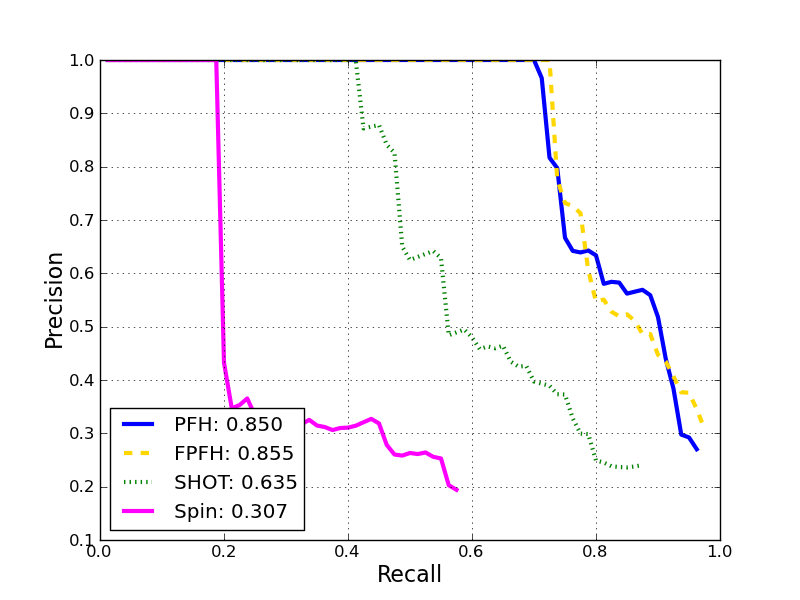
\includegraphics[width=0.45\linewidth]{../figures/PSB/PFH-FPFH-SHOT-SPIN_IMAGE_pr.png}
} \subfloat[Cumulative rank histogram shows the proportion of trials in which the correct result was fetched by the features in the initial stage.]{
\label{fig:PSB_rankhist}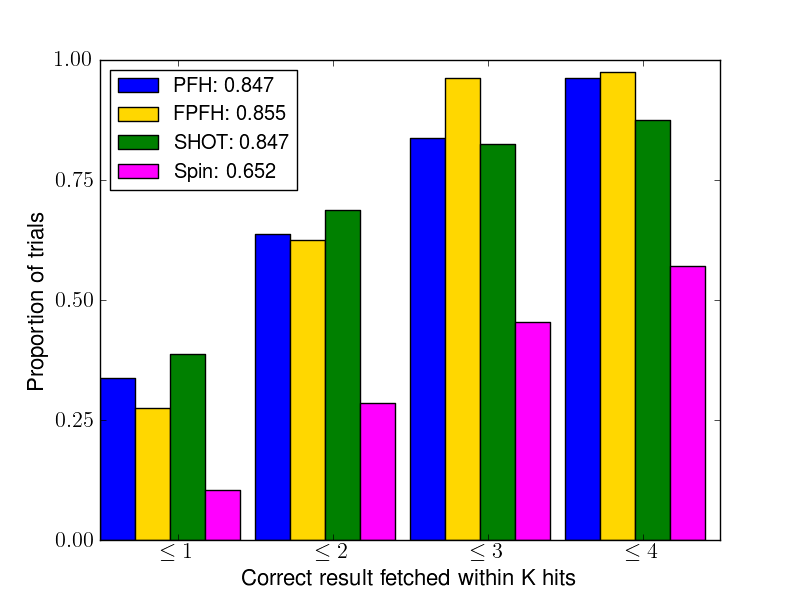
\includegraphics[width=0.45\linewidth]{../figures/PSB/PFH-FPFH-SHOT-SPIN_IMAGE_rankhist.png}
} \\
  \subfloat[PFH]{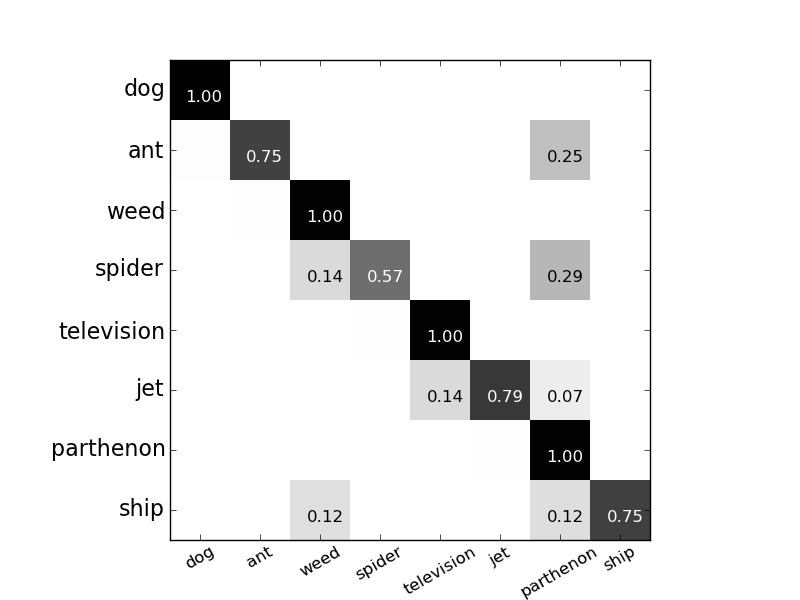
\includegraphics[width=0.45\linewidth]{../figures/PSB/PFH_confmat.png}}
  \subfloat[FPFH]{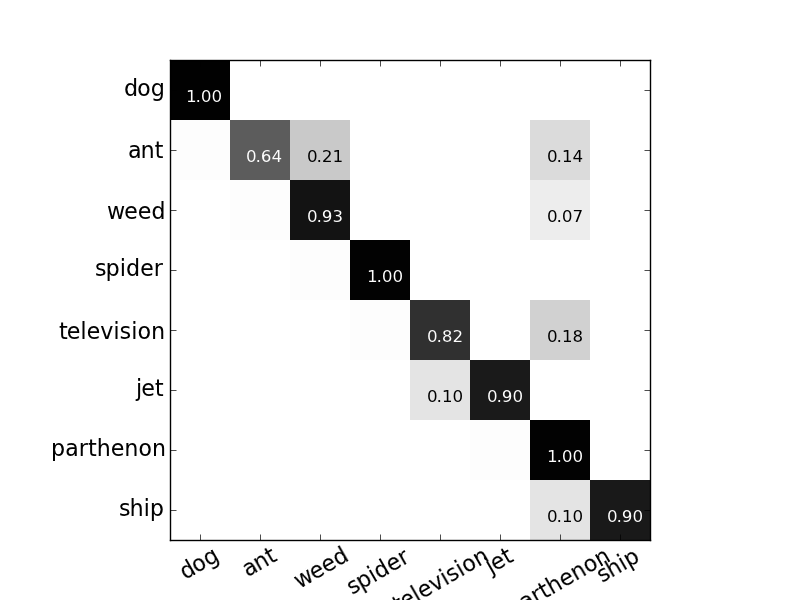
\includegraphics[width=0.45\linewidth]{../figures/PSB/FPFH_confmat.png}}\\
  \subfloat[SHOT]{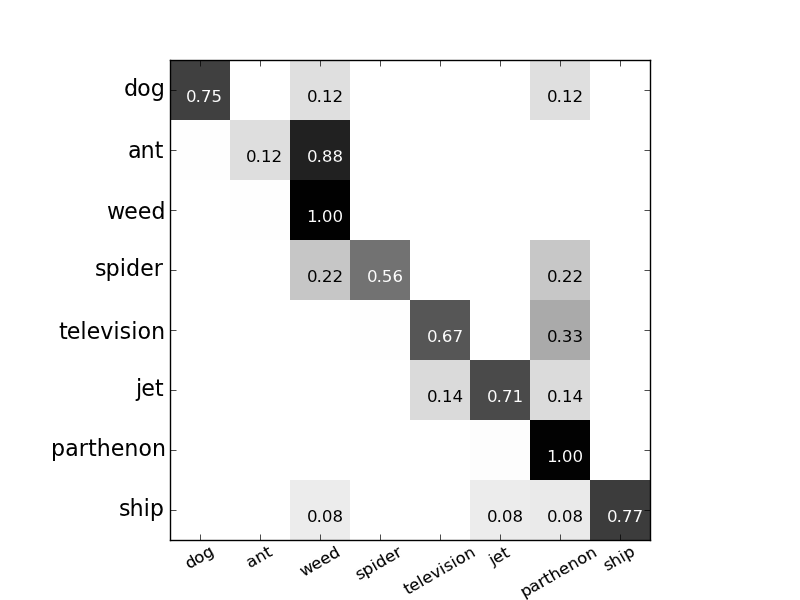
\includegraphics[width=0.45\linewidth]{../figures/PSB/SHOT_confmat.png}}
  \subfloat[Spin Image]{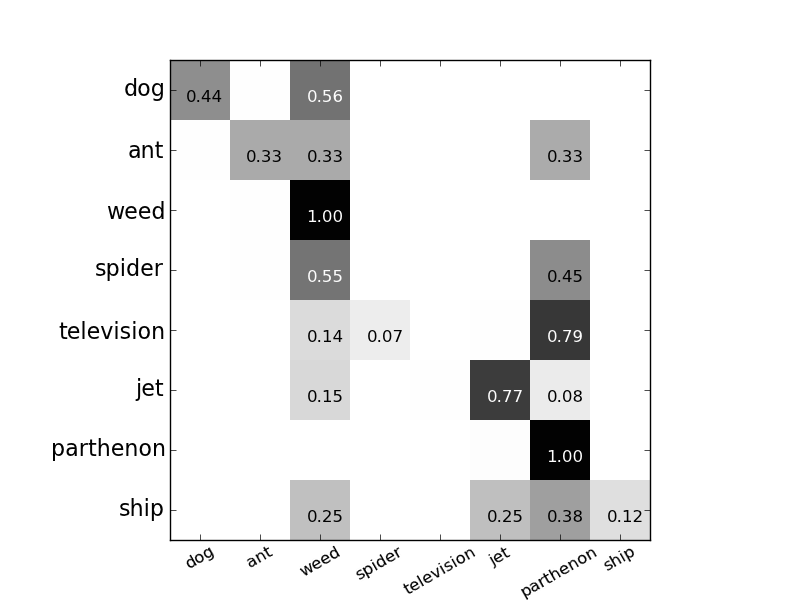
\includegraphics[width=0.45\linewidth]{../figures/PSB/SPIN_IMAGE_confmat.png}}
  \caption{Dashboard for the accuracy-related performance of the different features on the Princeton Shape Benchmark dataset.}
  \label{fig:PSB_dashboard}
\end{figure*}

\begin{figure*}[thpb]
\centering
\subfloat[Total time spent in training.]{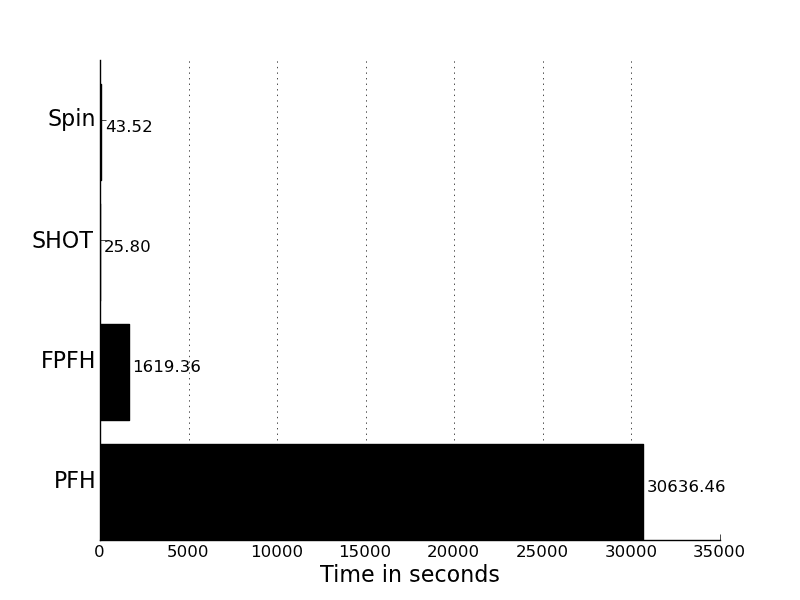
\includegraphics[width=0.45\linewidth]{../figures/PSB/PFH-FPFH-SHOT-SPIN_IMAGE_train_total.png}}
\subfloat[Total time spent in testing.]{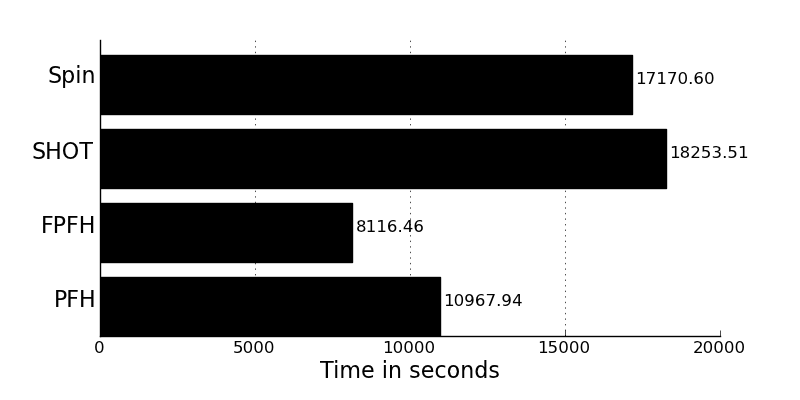
\includegraphics[width=0.45\linewidth]{../figures/PSB/PFH-FPFH-SHOT-SPIN_IMAGE_test_total.png}} \\
\vspace{1em}
\subfloat[Breakdown of where time is spent in the testing phase.]{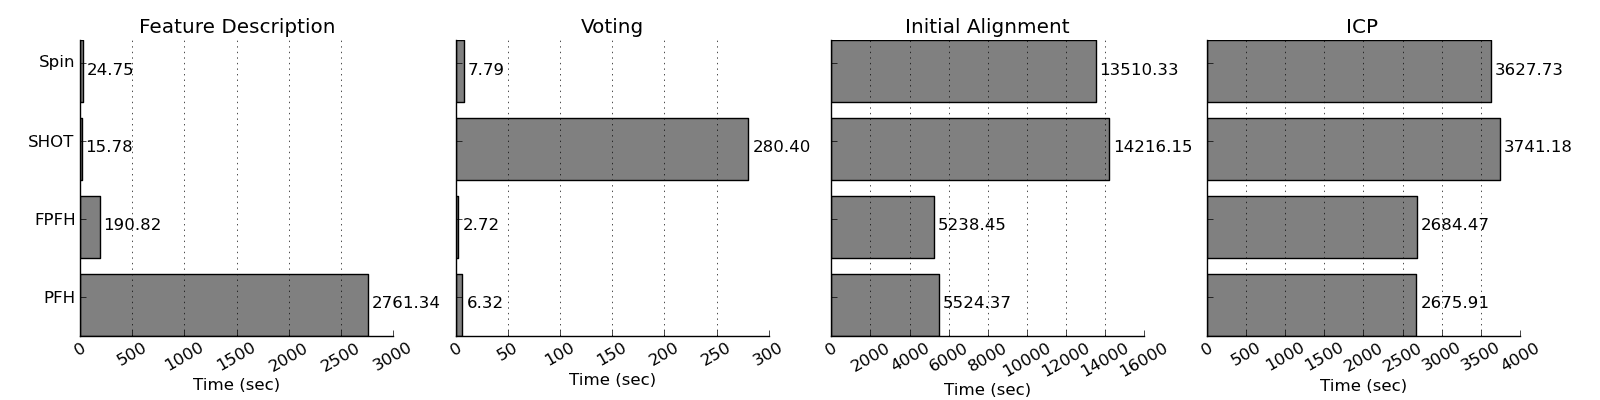
\includegraphics[width=0.95\linewidth]{../figures/PSB/PFH-FPFH-SHOT-SPIN_IMAGE_timing_test_panel.png}} 
\caption{Timing results on the Princeton Shape Benchmark dataset.}
\label{fig:PSB_timing}
\end{figure*}

%
\begin{table*}
\centering
\begin{tabular}{m{0.08\textwidth} m{0.45\textwidth} m{0.45\textwidth}}
  & \begin{center} Confusion Matrix \end{center} & \begin{center} Cumulative Rank Histogram \end{center} \\
  PFH & 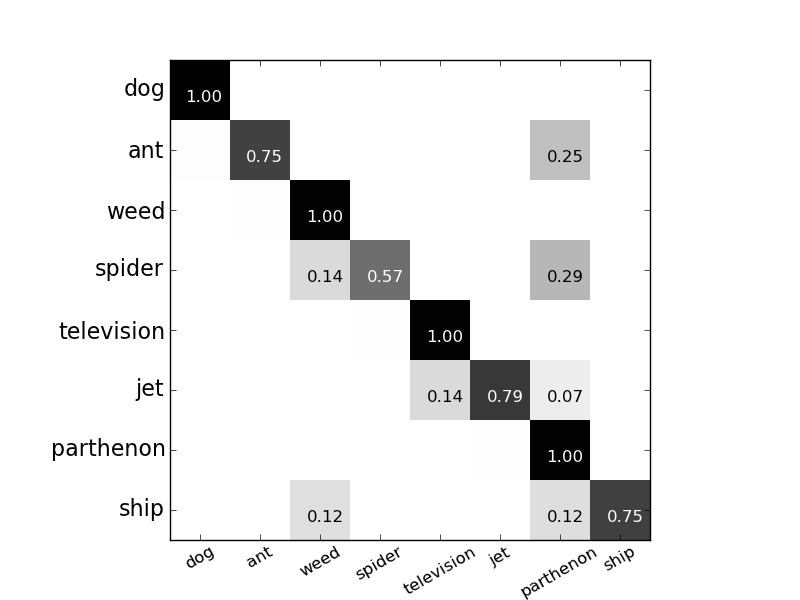
\includegraphics[width=0.45\textwidth,clip=true]{../figures/PSB/PFH_confmat.png} & 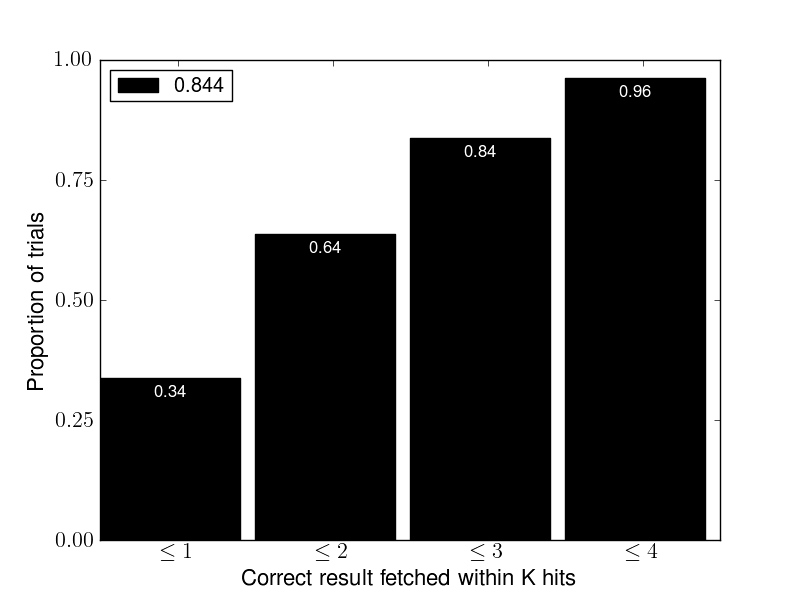
\includegraphics[width=0.45\textwidth,clip=true]{../figures/PSB/PFH_rankhist.png} \\
  FPFH & 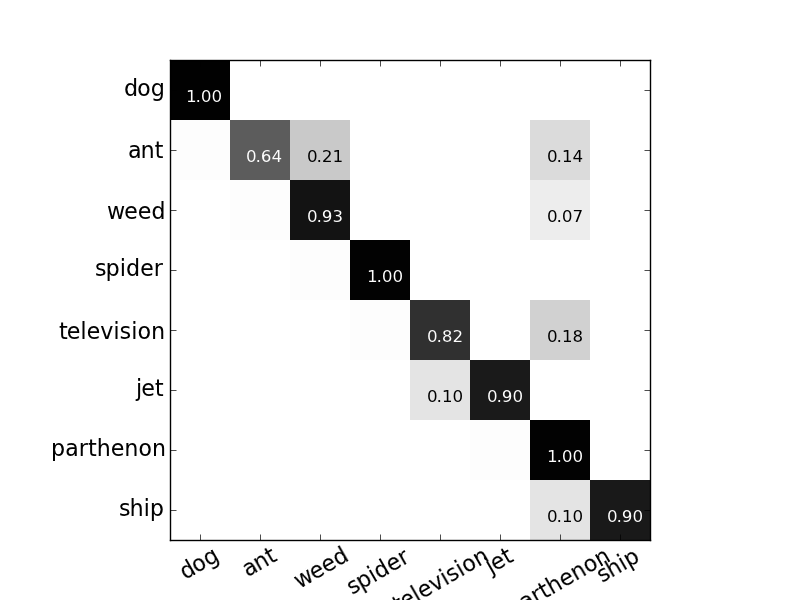
\includegraphics[width=0.45\textwidth,clip=true]{../figures/PSB/FPFH_confmat.png} & 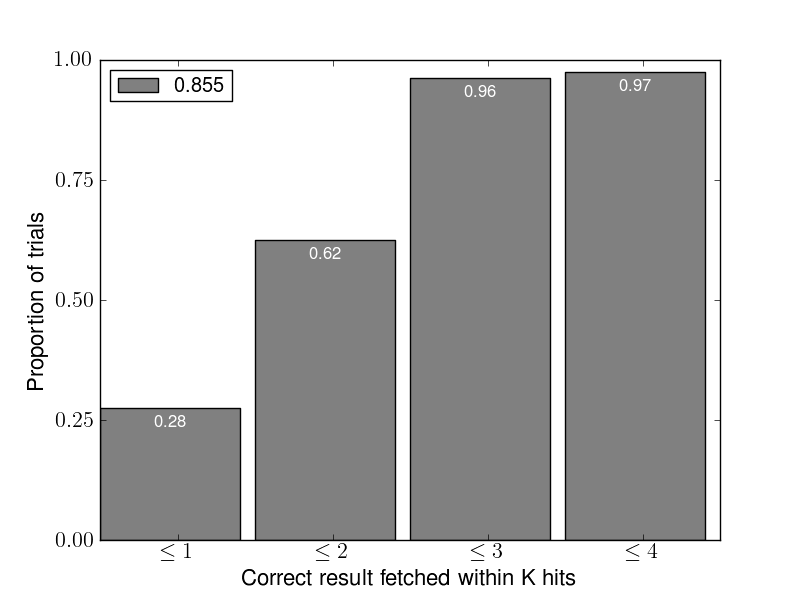
\includegraphics[width=0.45\textwidth,clip=true]{../figures/PSB/FPFH_rankhist.png} \\
  SHOT & 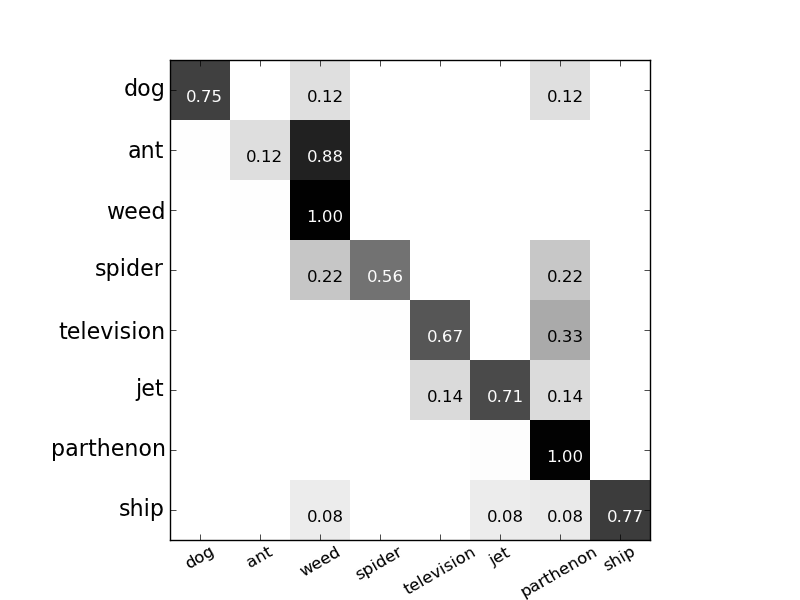
\includegraphics[width=0.45\textwidth,clip=true]{../figures/PSB/SHOT_confmat.png} & 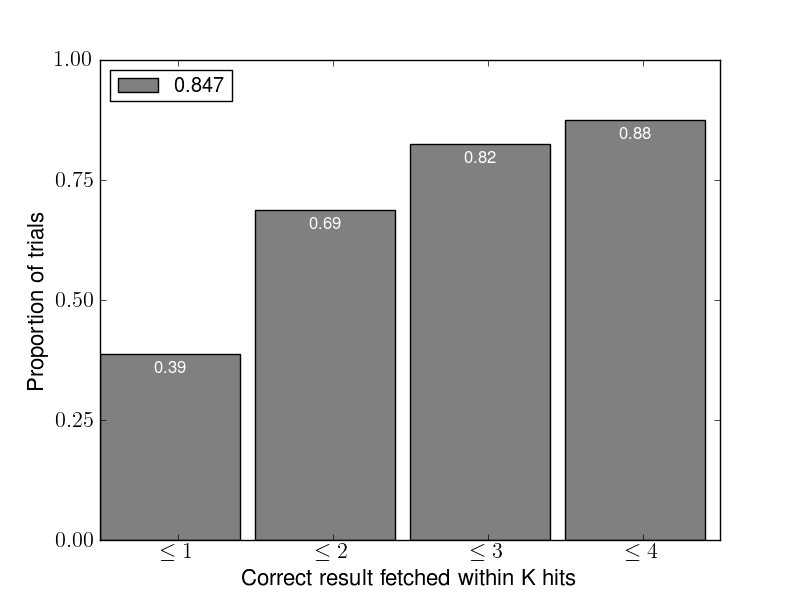
\includegraphics[width=0.45\textwidth,clip=true]{../figures/PSB/SHOT_rankhist.png} \\
  Spin Image & 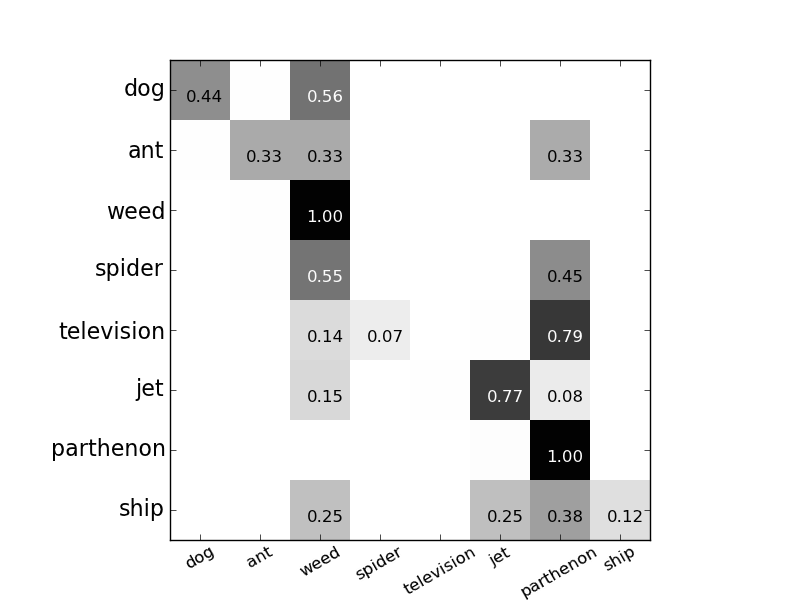
\includegraphics[width=0.45\textwidth,clip=true]{../figures/PSB/SPIN_IMAGE_confmat.png} & 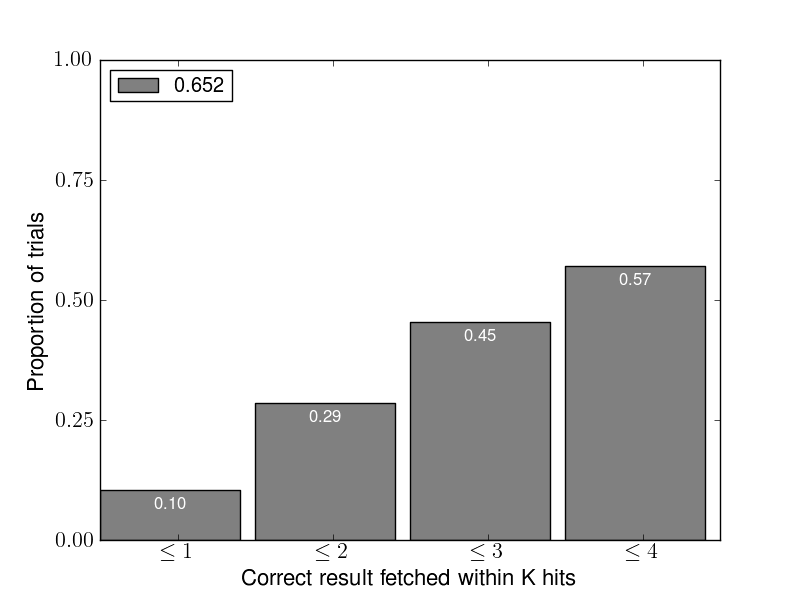
\includegraphics[width=0.45\textwidth,clip=true]{../figures/PSB/SPIN_IMAGE_rankhist.png} \\
\end{tabular}
\caption{A table arranging images}
\label{tab:gt}
\end{table*}

An additional important evaluation is the runtime performance of different methods.
This data allows focused work on fast feature extraction and on algorithms to speed up matching, such as locality-sensitive hashing \cite{Frome2004}.
Hence, we report timing results, split by the different stages of our pipeline, for all experimental conditions.
In all cases, the tests were run on a 2.50 GHz Intel Core2 Quad Q9300 with 4 GB of RAM.

* table per dataset

* features vs. metrics

* plots of the same data that's in the tables?

* confusion matrix figures

* table of timing results
